% ----------------------------------------------------------
% Introdução (exemplo de capítulo sem numeração, mas presente no Sumário)
% ----------------------------------------------------------

\chapter{Introdução}\label{intro}
\section{Conceitos Introdutórios e Problematização}
Com os avanços recentes na miniaturização de componentes eletrônicos de prateleira (COTS), construir 
satélites deixou de ser exclusividade de governos e grandes empresas apoiadas por governos, agora 
universidades, empresas menores e grupos entusiastas podem construir e lançar ao espaço em um ou dois 
anos pequenas espaçonaves de baixo custo, baixa potência com componentes de prateleiras prontos para 
uso \cite{Poghosyan2017}.

Está tecnologia vem permitindo que países em desenvolvimento e emergentes possam entrar no setor espacial, 
o desenvolvimento, operação e análise de dados dessas pequenas espaçonaves promovem e estimulam a educação 
científica em mais de 80 universidades em todo o mundo que possuem programas nessas áreas, estes programas 
ocasionam uma importante atividade comercial, com muitos desses projetos surgindo como projetos acadêmicos 
\cite{Woellert2011}. O padrão de um CubeSat de uma unidade (1U) e de 10 x 10 x 10 cm³, tendo seu peso 
limitado a 1,33 kg podendo ser composto por um ou mais unidades seguindo o mesmo padrão, este padrão foi 
inicialmente desenvolvido em 1999 pelos professores Jordi Puig-Suari na Cal Poly e Bob Twiggs na Universidade 
de Stanford, cada uma dessas espaçonaves pode ser lançadas ao custo de 50 a 200 mil dólares\cite{Selva2012}, 
este custo pode variar dependendo das tecnologias empregadas e plataforma de lançamento.

% \begin{figure}[H]
% 	\centering
% 	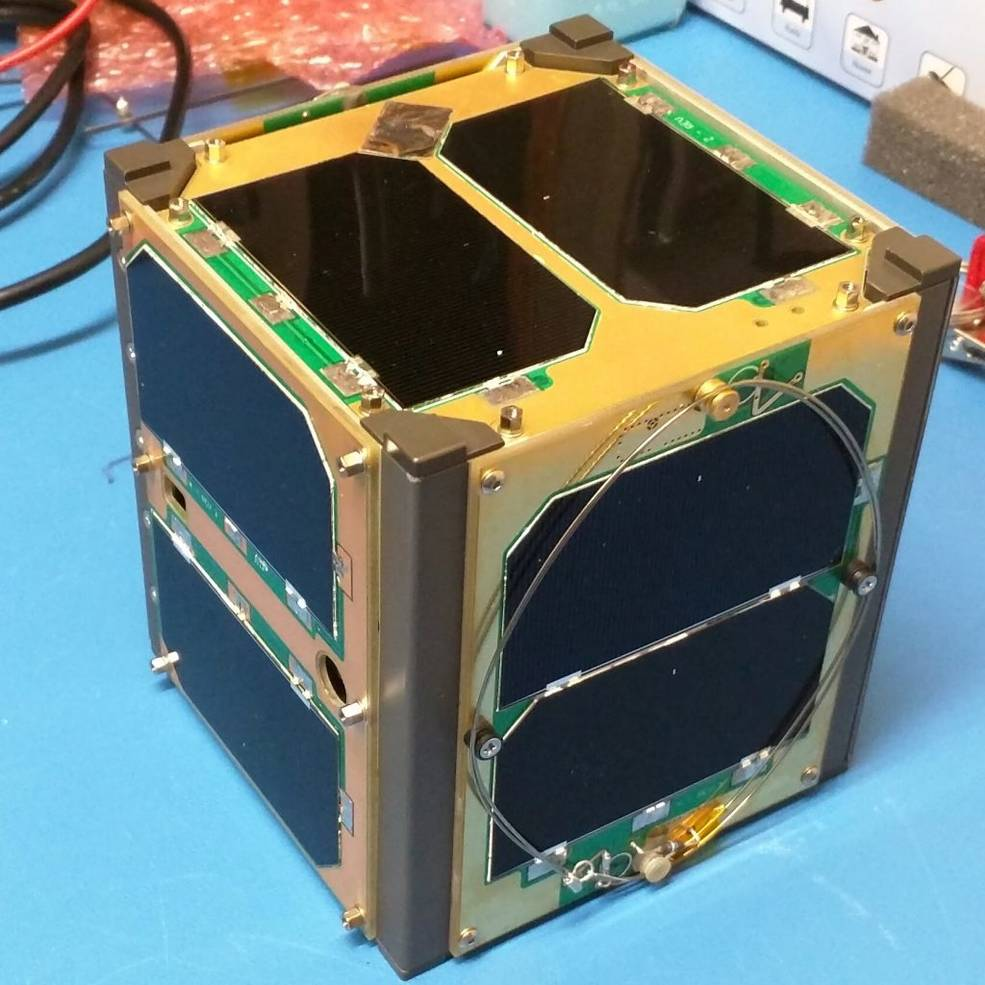
\includegraphics[width=15cm]{imagens/cubesat_nasa_image.jpg}
% 	\caption{CubeSat RadFxSat}
% 	Fonte: Portal "www.nasa.gov", The Radio Amateur Satellite Corporation (AMSAT) e Vanderbilt University.
% 	\label{fig: CubeSat RadFxSat}
% \end{figure}

A fim de diminuir custos estas plataformas podem ser construídas com tecnologias de código aberto. Os CubeSat's 
de código aberto populares possuem uma característica em comum, utilizam o sistema operacional de tempo real de 
código aberto FreeRTOS, pois além de ser um dos RTOS (Sistema operacional de Tempo Real) mais adotado para projetos e um dos mais populares segundo 
a \cite{Lynx}. E um dos RTOS com maior documentação e maior comunidade na internet, sendo um dos favoritos em 
projetos de código aberto por ter maior aceitação e entendimento do publico. O mesmo e pequeno, simples e confiável 
sendo amplamente usado na indústria de microeletrônica, sendo escrito em C com partes em assembler \cite{nicolas2019avaliaccao}.


Desta forma, pretendeu-se avaliar um novo sistema operacional de tempo real para a utilização do mesmo no 
desenvolvimento de CubeSats, visto que o projeto Zephyr. De acordo com \cite{nyffenegger2020connecting}destaca 
que o Zephyr RTOS é um sistema relativamente novo no mercado, destacando-se em sua construção pensada para operar 
em ambientes restritos a poucos recursos de memoria e consumo de energia, permitindo que aplicativos complexos 
sejam executados em dispositivos altamente limitados. É altamente modular, permitindo que os usuários configurem 
o funcionamento do sistema de acordo com as necessidades do projeto sem prejudicar os requisitos, entretanto 
por se tratar de um sistema novo, implica em ter um suporte difícil para iniciantes, exigindo um nível de 
habilidade alta na compreensão e configuração de sistemas Linux com Makefiles, um ponto destacado negativamente 
está na carência de resoluções de problemas na internet e documentação para iniciantes fraca de explicações, 
tornando a curva de aprendizado bastante íngreme. Utilizar Zephyr em um projeto de Cubesat não 
e uma ideia muito distante, abrindo uma janela de possíveis trabalhos na área que possam 
trazer grandes contribuições, possibilitando o surgimento deste trabalho.


Em \cite{Slacka} o autor destaca algumas dificuldades ao se desenvolver um sistema operacional para missões de 
cubesat, pois nem sempre o sistema poderá estar acessível a um operador humano, tornando a responsabilidade do 
software em tomar atitudes em tempo real mais desafiadoras, o sistema precisa ter confiabilidade e tolerância a 
falhas de software e hardware. Também informa que sistemas operacionais de tempo real como o 
FreeRTOS empregam muitas funcionalidades complexas e custosas que não necessariamente serão empregadas em uma 
missão de cubesat.


\section{Objetivos e Escopo de Pesquisa}
\subsection{Objetivos de Pesquisa}
Visto a exorbitante quantidade de dados provindo de sensores, somando a incerteza da qualidade de fabricação dos componentes eletrônicos de baixo custo disponíveis em ampla quantidade no mercado, torna o desenvolvimento para sistemas criticos que dependem da veracidade dos valores provindos dos sensores, ambiente assíncrono com múltiplas tarefas em simultâneo, complexos e custosos para as equipes de engenheiros de software, que utilizam de tempo para garantir a integridade e veracidades de todos os valores. 

Com isso em mente o trabalho aqui proposto se dispõem de construir uma biblioteca de código aberto, que disponibilizara funções adequadas para a filtragem de dados provindo de sensores em ambiente de tempo real com multitarefas, testando a coleta e filtragem de dados no processador dual core ESP32 no sistema operacional de tempo real \cite{Zephyr}.

\subsection{Objetivos secundários}
Os objetivos secundários a serem alcançados são:
\begin{itemize}
\item Realizar uma revisão bibliométrica de trabalhos que utilizam de métodos probabilísticos para filtragem de dados de sensores
\item Disponibilizar o código de forma aberta a comunidade, para que possa ser utilizado por qualquer outro interessado em tratar dados de sensores em ambiente de multitarefas
\item Escrever funções de filtragem utilizando os métodos de Desvio padrão e Intervalo de confiança
\end{itemize}


\subsection{Escopo da Pesquisa}
O escopo desta pesquisa abrange teste de diversos critérios de \cite{Raymundo} e \cite{Garcia} utilizando linguagem C++ no Chip ESP32 da fabricante Espressif. Neste trabalho serão levadas em consideração apenas detalhes ligados ao sistema operacional empregado na missão de um CubeSat, sendo desconsiderada detalhes mais técnicos de um voo espacial, como problemas de inversão de bit e perda de dados por culpa de radiação e outros problemas específicos. Assim, em um primeiro momento considerou-se avaliar apenas a performance em um único chip fora de um chassi e estrutura de uma espaçonave.


\section{Justificativas}
A comunidade de desenvolvimento de CubeSats educacionais de código aberto utilizam em sua grande maioria de 
poucos RTOS disponíveis no mercado, exemplo o FreeRTOS, em virtude de sua já confirmada performance e garantia 
em embarcada, considerando os poucos recursos para empregar um sistema ainda não validado na arquitetura do 
projeto.
Visto que o ESP32 é um chip muito popular e já validado em viagens espaciais, destaca-se que 
a contribuição para o setor, por meio desta pesquisa, 


% Validar isso
será a avaliação de um sistema novo e que promete ser mais 
eficiente em fatores como memoria, espaço e energia, sendo que o mesmo ainda não foi validado em uma missão 
real, 



assim então economizando tempo e dinheiro das equipes e universidades que usufruem de projetos de CubeSat.


\section{Organização do Trabalho}
% Inserir resultados
Este trabalho está organizado da seguinte forma, para o capítulo 1 apresentou-se a introdução da 
pesquisa, com dados e justificativas baseadas na bibliografia de suas áreas, contendo 
também os objetivos do trabalho, além do escopo e justificativas. Já no capítulo 2 apresenta-se 
uma revisão bibliométrica acerca dos trabalhos relacionados e do escopo deste projeto. O 
capítulo 3 contém aspectos da metodologia adotada e os requisitos necessários, com o capítulo 
4 possuindo a definição do experimento e de seus criterios detalhadamente, que por ultimo 
contendo o capítulo 5 traz as conclusões retiradas desta pesquisa, com suas possiveis contribuições 
e beneficios para a sociedade, comunidade científica e de desenvolvimento de CubeSats.

% Texto corrido